% !TEX root = ../Thesis.tex
\acresetall
\myChapter{Outlook}\label{ch:outlook}
\begin{flushright}{\slshape    
		So Long, and Thanks for All the Fish} \\ \medskip
    --- \defcitealias{Adams1984}{Douglas Adams}\citetalias{Adams1984} \citep{Adams1984}
\end{flushright}
\vspace{52mm}

\begin{itemize}
	\item Sebastien -> multimodal
	\item Skeletonization
	\item Structural Analysis of the lung
	\item Acinar Growth
\end{itemize}

\renewcommand{\imsize}{\linewidth}
\begin{figure}[ht]
	\centering
	\pgfmathsetlength{\imagewidth}{\imsize}%
	\pgfmathsetlength{\imagescale}{\imagewidth/1541}%
	\begin{tikzpicture}[x=\imagescale,y=-\imagescale]
		%\def\x{952} % scalebar-x at golden ratio of x=1541px
		%\def\y{588} % scalebar-y at 90% of height of y=653px
		\def\x{1300} % scalebar-x at golden ratio of x=1541px
		\def\y{400} % scalebar-y at 90% of height of y=653px
		\node[anchor=north west, inner sep=0pt, outer sep=0pt] at (0,0) {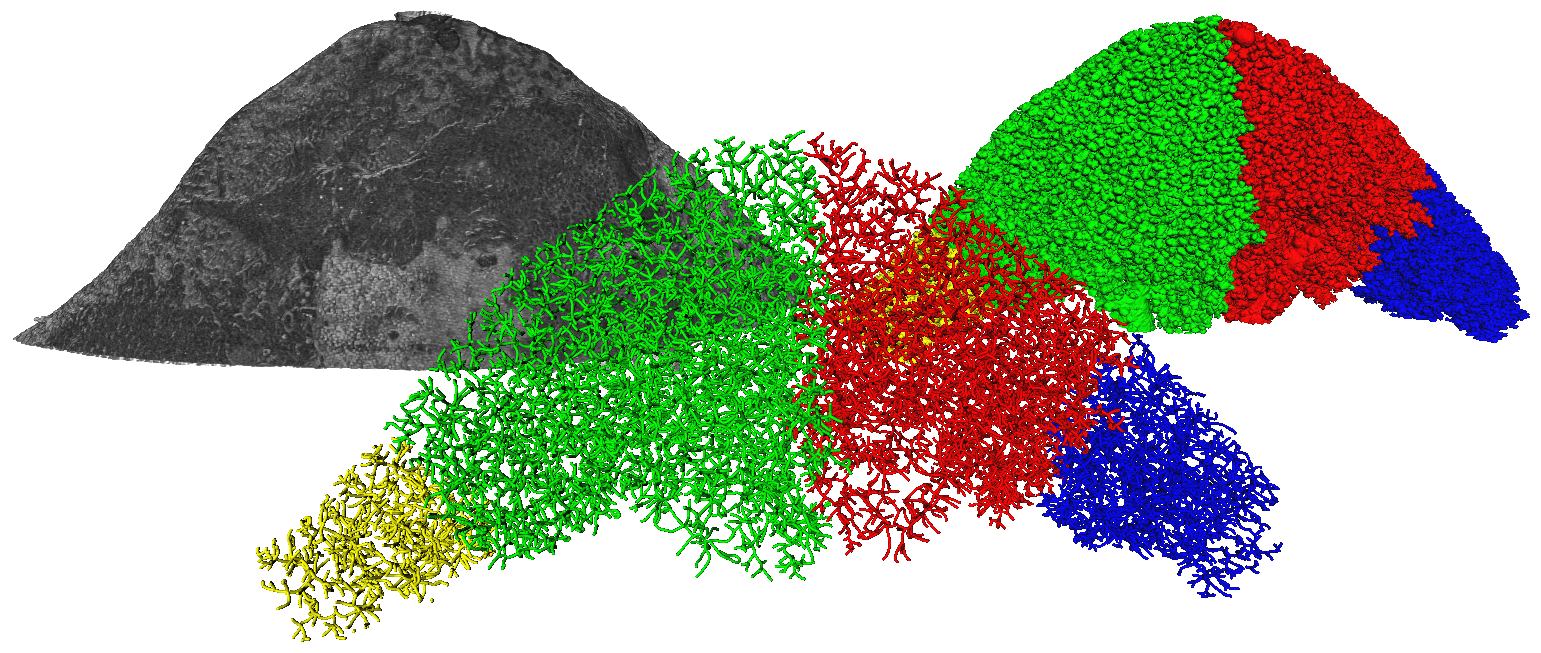
\includegraphics[width=\imagewidth]{img/R108C21b-skeleton}};
		% 796px = 4.0138mm > 100px = 504um > 99px = 500um, 20px = 100um
		%\draw[color=red,|-|,thick] (11,341) -- (807,339) node [sloped,midway,above] {\SI{4.0138}{\milli\meter} (2712px)};
		\draw[|-|,thick] (\x,\y) -- (\x+99,\y) node [midway, above] {\SI{500}{\micro\meter}};
	\end{tikzpicture}%
	\caption{Visualization of rat lung sample obtained at postnatal day 21. Left: Three-dimensional view of the sample, Right: Four independent airway segments. Foreground: Extracted airway skeletons of the independent airways. The yellow skeleton contains \num{1133}, the green \num{7288}, the red \num{6513} and the blue skeleton \num{3278} nodes.}
	\label{fig:skeleton}
\end{figure}

\renewcommand{\imsize}{0.618\linewidth}
\begin{figure}
	\centering
	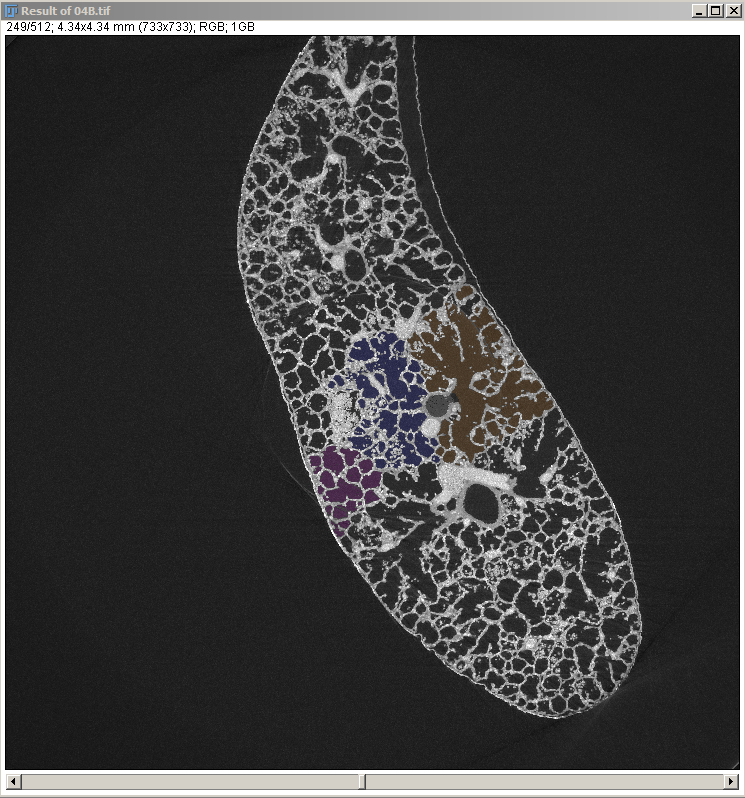
\includegraphics[width=\imsize]{img/Acinus_Overlay}
	\caption{Acinus Overlay}
	\label{fig:acinus overlay}
\end{figure}